%%
%% Template chap1.tex
%%

\chapter{Preliminaries}
\label{cha:Preliminaries}

In this chapter, we briefly introduced preliminary backgrounds of the techniques we used through out our study. We started by a classic machine learning model called neural networks. Then several variations of neural networks serving different purposes were compared, which are convolutional neural networks, auto-encoders, convolutional auto-encoders, respectively. After that we looked at another unsupervised feature extraction and dimensionality reduction method called principle component analysis, as well as its application in whitening. Then we discussed a type of probabilistic graphical models called Markov random fields, and how it can be used to express the dependency between variables. Finally, we introduced two of the most concerned topics in the field of computer vision, namely image segmentation and 3D reconstruction.

\section{Neural Networks}
\label{sec:Neural Networks}
A commonly used model for regression and classification problems takes the form of
\begin{equation}
	y(x) = f(W \Phi (x))
\end{equation}
where $f(\cdot)$ is an activation function, and $\Phi(x)$ are the basis functions, which can also be interpreted as a set of features. 

While many models suffer from the limitation that the basis function should be fixed before the training data set is observed, neural networks provide a way of learning features from data implicitly by making making the basis functions $\Phi_j(x)$ depend on parameters which are allowed to be adjusted during the training step.
\subsection{Network functions}
\label{sec:NN functions}

A typical neural network model is composed of a series of layers. Each layer constructs $M$ linear combinations of the input variables from its previous layer, and transforms them using an activation function in the form
\begin{equation}
	h = \sigma(Wx+b) 
\end{equation}
where parameters $W$ are referred to as the weights of input units, $b$ is the bias term, and $\sigma(\cdot)$ is a differentiable nonlinear function. 

For binary classification problems the logistic sigmoid function in the form
\begin{equation}
	y = \sigma(a) = \frac{1}{1+\exp(-a)}
\end{equation}
is used for output units, so that we can interpret the output as the conditional probability with respect to a Bernoulli distribution, and the following properties are satisfied.
\begin{equation}
	0<\sigma(a)<1, 
\end{equation}
\begin{equation}
	\sigma(a) = 1-\sigma(-a). 
\end{equation}
Similarly for multiclass problems, a softmax activation function is used, which takes the form
\begin{equation}
	y_k(x) = \frac{\exp(a_k)}{\sum\nolimits_j \exp(a_j)},
\end{equation}
where $a_k$ is the pre-activation value for the $k$-th output unit.

For instance, the overall network function of a two-layer neural network can be given as 
\begin{equation}
	\label{nn2eq}
	y = \sigma_2(W^2\sigma_1(W^1x+b^1)+b^2).
\end{equation}
Its corresponding architecture is illustrated in Figure \ref{nnfig}~\cite{bishop2006pattern}.

\begin{figure}[h!]
  \centering
  \label{nnfig}
  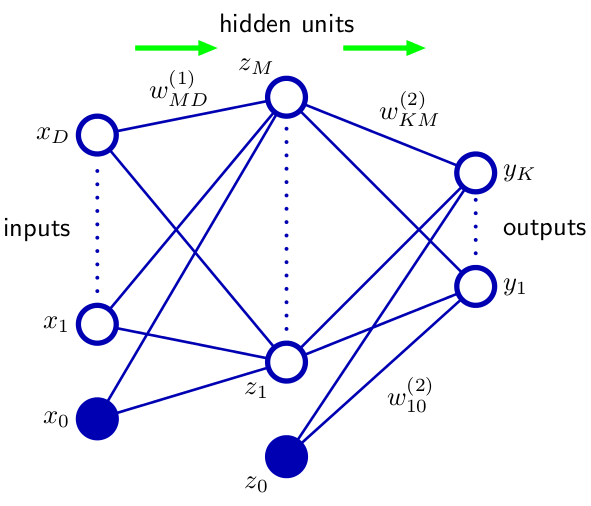
\includegraphics[width=0.7\textwidth]{pics/nn.png}
  \caption{Network architecture for the two-layer neural network corresponds to \ref{nn2eq}. Weights associated with node $x_0$ correspond to term $b^1$, weights associated with node $z_0$ correspond to term $b^2$. }
\end{figure}

It is shown that multilayer feedforward networks defined this way can approximate any arbitrary function to any desired degree of accuracy, provided sufficiently many hidden units are available~\cite{hornik1989multilayer}.

\subsection{Network training}
\label{sec:NN training}
Neural networks can be trained by minimizing an error function, which corresponds to the maximum-likelihood estimation (MLE) with regard to certain probabilistic assumptions. In terms of classification problems, the cross-entropy error function of the form
\begin{equation}
	E(\theta) = -\sum\limits_{n=1}^N\sum\limits_{k=1}^Kt_{kn}\ln y(x_n)
\end{equation}
is used, where $K$ is the number of mutually exclusive classes, and $t_n$ is a vector of zeros and ones indicating the target class.

We can apply the stochastic gradient descent algorithm to find a good set of parameters that yields a reasonable amount of errors. The gradient information required with regard to relevant parameters can be evaluated efficiently by error backpropagation~\cite{rumelhart1985learning} in the context of neural networks.

\section{Convolutional Neural Networks}
\label{sec:Convolutional Neural Networks}

In natural images, pixels that are spatially nearby are highly correlated. The main disadvantage of using neural networks for image classification is it ignores the topology of the input by constructing fully-connected networks. Moreover, fully-connected architectures are associate with a large number of parameters given high-dimensional data, which is prone to overfitting. Therefore convolutional neural networks (CNN) were introduced as a way to extract local, translation invariant features, and limiting the number of parameters substantially at the same time~\cite{lecun1995convolutional}.


\subsection{Architectural properties}
\label{sec:Architectural properties}

Convolutional neural networks incorporate three architectural ideas on top of neural networks described previously, which are local receptive fields, shared weights, and pooling and sub-sampling. In following discussions we are going to use the terms ``pixel'' and ``channel'' for better illustration in the context of image classification.

\subsubsection{Local receptive fields}
\label{sec:Local receptive fields}
In convolutional neural networks, each pixel of a channel receives inputs from a set of pixels located in a small neighborhood in each channel of previous layer, namely the receptive fields. The output is computed by taking discrete convolution of the receptive fields and kernel matrices (parameters to be tuned), then followed by an activation function. 

\subsubsection{Shared weights}
\label{sec:Shared weights}
The same set of kernel matrices is shared between receptive fields in different locations of the image. Such approach enables us to extract local features (e.g., oriented edges, end-points, corners) in the scope of the size of kernel matrices. Channels of hidden layers are also referred to as feature maps as each of them represents the outcome obtained using different features (kernel matrices). Separate kernel matrices are used between different input or output channels. For example, a layer with $m$ feature maps and $n$ channels will incorporate a number of $m*n$ kernel matrices.

\subsubsection{Pooling and sub-sampling}
\label{sec:Pooling and sub-sampling}
Pooling and sub-sampling refer to the operations that are performed on non-overlapping neighbourhoods. Information of each neighbourhood are usually aggregated in some way to obtain a single value. The benefit of pooling is, the resolution of feature maps are reduced, as well as the sensitivity of the output to shifts and distortions. For instance, the max pooling operation on $2$ by $2$ non-overlapping neighbourhoods will resulting a feature map of $1/4$ of its original size, where each element takes the max value of its corresponding neighbourhood.

\subsubsection{Network architecture}
\label{sec:Network architecture}
In practice, a convolutional layer is often followed by a pooling or sub-sampling layer. By stacking such structures repeatedly, we are able to extract effective higher order features. An example architecture of convolutional neural networks are shown in Figure \ref{cnnfig} by~\cite{lecun1995convolutional}.

\begin{figure}[h!]
  \centering
  \label{cnnfig}
  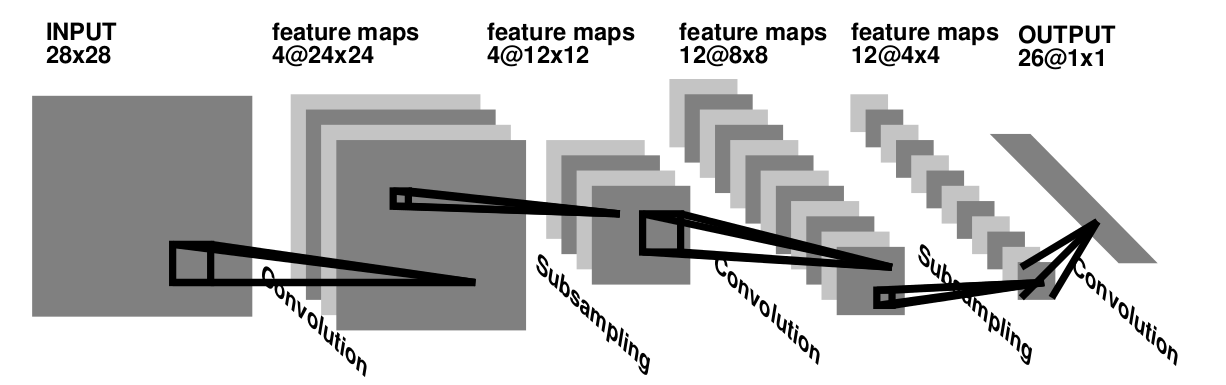
\includegraphics[width=\textwidth]{pics/cnn.png}
  \caption{The first layer is a convolutional layer with $4$ feature maps and $5$ by $5$ kernels, the second layer is a $2$ by $2$ sub-sampling layer, the other layers are of similar properties as illustrated.}
\end{figure}

\subsection{Network functions}
\label{sec:CNN functions}
Based on the architecture properties described above, for a $N$-channel input $x$ the $k$-th feature map of the next convolutional layer is given by
\begin{equation}
	h_k(x) = \sigma(\sum\limits_{n=1}^Nx_n\ast W^{nk} + b^k).
\end{equation}
For a pooling or sub-sampling layer, the output depends on the operation specified by that layer. For example, if a $p$ by $q$ max pooling layer is used, the pixel at position $(i,j)$ of a feature map is then given by
\begin{equation}
	\label{submx}
	y_{ij} = \max\limits_{m,n}x_{mn},
\end{equation}
which subjects to the constraint that
\begin{equation}
	m,n\in R_{ij}
\end{equation}
where $R_{ij}$ is a $p$ by $q$ non-overlapping at the $(i,j)$ position.
Output activation functions, error functions of convolutional neural networks are similar to neural networks described previously.

\subsection{Network training}
\label{sec:CNN training}

Let $E$ be the error function, for discrete convolution operation $y=x\ast W$, its partial derivatives with respect to $x$ is given by 
\begin{equation}
	\frac{\partial E}{\partial x} = \frac{\partial E}{\partial y}\bar{\ast} w, 
\end{equation}
where $\bar{\ast}$ denotes the opposite way of performing convolutions of $*$ (e.g., if $\ast$ is the valid convolution, $\hat{\ast}$ should be the full convolution). Its partial derivatives with respect to $W$ is 
\begin{equation}
	\frac{\partial E}{\partial W}   = \frac{\partial E}{\partial y} \ast\tilde{x},
\end{equation}
where $\tilde{x}$ denotes a matrix given by $x$ with its rows and columns flipped. Having defined the partial derivatives for discrete convolution, we can use error backpropagation and gradient based methods for training convolutional neural networks. 

\section{Auto-encoders}
\label{sec:Auto-encoders}
Because the amount of available labels are very limited in many situations, it is important to exploit the usability of unlabeled data. Auto-encoders is an unsupervised learning approach aimed at learning hidden properties of unlabeled data. It is based on neural networks, and can leverage the utility of neural networks in turn.

\subsection{Network architecture}
\label{Network architectur}
Auto-encoders are essentially neural networks trained to reproduce its input at the output layer. By doing this it tries to learn a distributed representation that captures the main factors of variation in the data and hence remove input redundancies~\cite{bengio2009learning}. 

Auto-encoders first transform the high-dimensional data into a low-dimensional representation in the form of
\begin{equation}
	h(x) = \sigma(Wx+b).
\end{equation}
Then it tries to recover the data from the code via a similar ``decoder'' network, which is given by
\begin{equation}
	\hat{x} = \sigma(W'x+c).
\end{equation}
The two parameter sets $W$ and $W'$ are usually made to share the same weights of the form 
\begin{equation}
	W' = W^T
\end{equation}
so that the network follows the same manner for encoding and decoding steps.

A typical architecture and its reconstruction result are illustrated in Figure \ref{aefig} by~\cite{lemme2010efficient}.  
\begin{figure}[h!]
  \centering
  \label{aefig}
  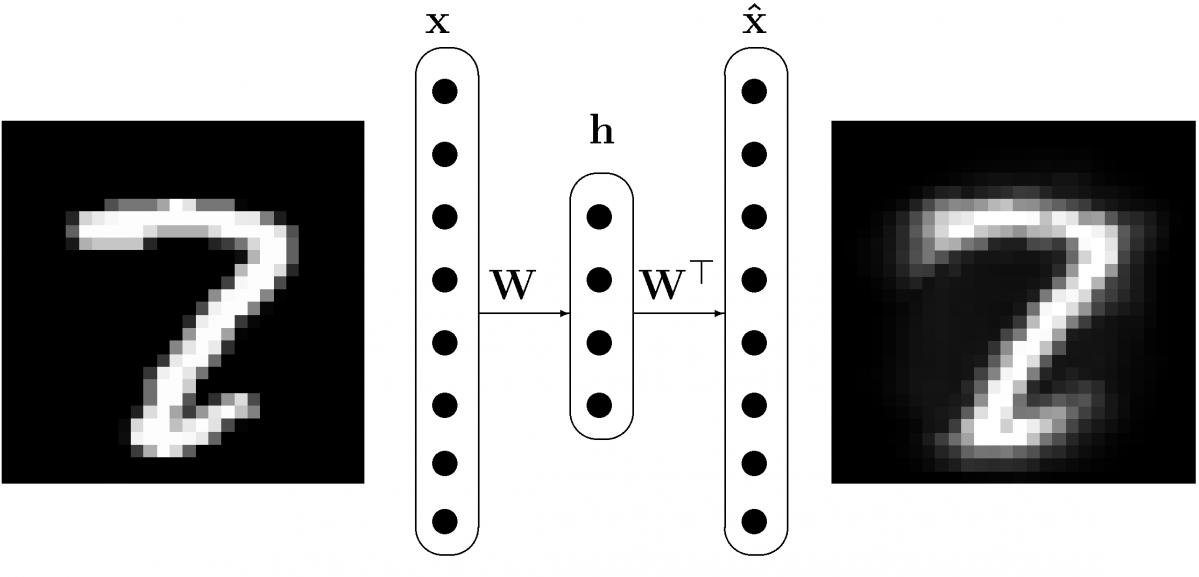
\includegraphics[width=0.8\textwidth]{pics/ae.png}
  \caption{ A typical auto-encoder network with tied weights $W$ and $W^T$, input image $x$ is shown in the left, its corresponding reconstructed image $\hat{x}$ is shown in the right.}
\end{figure}

\subsection{Network training}
\label{AE training}
Auto-encoders can be trained by minimizing the difference between the original data and its reconstruction. Since image pixels are numerical data, we can use sum of squared errors as our error function, which takes the form
\begin{equation}
	\label{aeerr}
	E(\theta) = \frac{1}{2n}\sum\limits_{i=1}^n(\hat{x_i}-{x_i})^2
\end{equation}
where $n$ is the number of data points.

The required gradients are obtained by using the chain rule to backpropagate error derivatives first through the decoder network and then through the encoder network~\cite{hinton2006reducing}. In particular, if weights are shared between encoding and decoding steps, $W$ and its transpose appears twice in the network. Thus the gradient with regard of $W$ is a sum of two gradients, which is given by
\begin{equation}
	\frac{\partial E}{\partial W} = (\frac{\partial E}{\partial \hat{x}}h)^T +  \frac{\partial E}{\partial h}x.
\end{equation}
Knowing the gradient information, the weights of the encoder network can be tuned by performing gradient descent in the same fashion as neural networks.

\subsection{Denoising Auto-encoders}
\label{Denoising Auto-encoders}
One problem of this approach is, if the dimension of hidden representation is greater than that of input data, the auto-encoder could potentially just learn the identity function, for the purpose of good reconstruction. 
The denoising auto-encoder is a variant of auto-encoder that addresses thsi issue by adding stochastical noise to the input data and trying to recover the original data~\cite{bengio2009learning}. 

The error function \ref{aeerr} with noiseless input can be applied directly to denoising auto-encoders. It can be proved that it raises a lower bound on the likelihood of several generative models~\cite{vincent2008extracting}.

\section{Convolutional Auto-encoders}
\label{sec:Convolutional Auto-encoders}
Interesting features can be extracted using denoising auto-encoders. However it assumes that pixels are independent input features, which makes it not suitable enough for processing natural images. Moreover a large number of parameters is required when when applied on high dimensional data. This will increase the non-convexity of error functions, and hence will increase the running time and difficulty in training.

Since convolutional neural networks often excels in image classification problems, convolutional auto-encoders were introduces based on the same architectural ideas. As a result, it is capable of learning local features in an unsupervised way, and scales well to high-dimensional input data since the number of free parameters becomes independent of the input dimensionality~\cite{masci2011stacked}.

\subsection{Network functions}
\label{Network functions}
Similar to general purpose auto-encoders, the aim of convolutional auto-encoders is to obtain a good reconstruction of input data from a set of hidden feature maps. It follows the similar mechanism as general purpose auto-encoders, and applies symmetric convolutional neural network architectures for encoding and decoding.

The network functions of convolutional auto-encoders differ from general purpose auto-encoders as it incorporates discrete convolutions. For a encoding convolutional layer, the $k$-th feature map of the latent representation is given by
\begin{equation}
	h_k(x) = \sigma(\sum\limits_{n=1}^Nx_n\ast W^{nk} + b^k)
\end{equation}
where $x$ is the input data and $N$ is the number of channels of $x$. In the corresponding deconding stage, the reconstruction is obtained using
\begin{equation}
	\hat{x}_n = \sigma(\sum\limits_{k=1}^Kh_k\bar{\ast} \tilde{W}^{nk} + c^n)
\end{equation}
where $\tilde{W}^{nk}$ identifies the matrix after flipping both dimensions of $W^{nk}$, and $\bar{\ast}$ identifies the opposite way of performing discrete convolution in the encoding step.

In convolutional neural networks, a pooling and sub-sampling layer is often applied to extract translation invariant features. Similarly a max pooling layer that eliminates all non-maximal values in non overlapping neighbourhoods in the form of
\begin{equation}
    y_{ij} = 
	\begin{cases}
    		m_{ij},& \text{if } m_{ij} = x_{ij}\\
    		0,              & \text{otherwise}
	\end{cases}
\end{equation}
where $m_{ij}$ is the maximum value of the belonging non-overlapping subregion of $x_{ij}$ defined in \ref{submx}.

By erasing non-maximal values we can acquire a sparse hidden representation which decreases the average number of features contributing to the decoding of each pixel, hence forces features to be more broadly applicable. Consequently, a max pooling layer will reduce the necessity of regularization over weights and stochastic noise over input data~\cite{masci2011stacked}.

\subsection{Network training}
\label{CAE training}
The error function defined in \ref{aeerr} is suitable for convolutional auto-encoders as well. Error backpropagation and stochastic gradient decent are also applicable for evaluating gradients and minimizing error functions. Since the weight matrices $W$ affects both the encoding and decoding stage, the corresponding gradient can be given as a summation of two gradient in the from of
\begin{equation}
\label{caeeq}
	\frac{\partial E}{\partial W^{nk}} = \widetilde{\frac{\partial E}{\partial \hat{x}_n}\ast h_k} +  \tilde{x_n}\ast\frac{\partial E}{\partial h_k}
\end{equation}
where $\frac{\partial E}{\partial h_k}$ and $\frac{\partial E}{\partial \hat{x}_n}$ are the partial derivatives of the hidden representation and the reconstruction output.


\section{Principal Component Analysis}
\label{sec:Principal Component Analysis}
Principal component analysis (PCA) is a commonly used method for dimensionality reduction. It can be defined as the orthogonal projection of the data onto a subspace of lower dimensionality, where the variance of projected data is maximized. Such subspace can represent a set of uncorrelated factors along which the data varies the most, hence it can also be used as a method for unsupervised feature extraction. 

\subsection{Maximum variance}
\label{Maximum variance}
We first begin with the case where the dimensionality of the subspace equals to one. For a given data set $x$, our goal is to find an orthogonal projection vector $u_1$ that maximizes the variance $v_1$ of $u_1^Tx$. 

The covariance matrix of the data is defined by
\begin{equation}
	S = \frac{1}{N}\sum\limits_{n=1}^N(x_n-\bar{x})(x_n-\bar{x})^T
\end{equation}
where $N$ is the number of data points, and $\bar{x}$ is the data set mean given by
\begin{equation}
	\bar{x} = \frac{1}{N}\sum\limits_{n=1}^Nx_n.
\end{equation}
Therefore the variance of projected data $V_1$ is given by
\begin{equation}
	v_1 = u_1^TSu_1.
\end{equation}

Because we need $u_1$ to be an orthogonal projection to ensure the bases of the subspace are linearly independent, $u_1$ needs to satisfy the condition 
\begin{equation}
	u_1u_1^T=I
\end{equation}
where $I$ is the identity matrix. 

It can be proved that the value of $u_1$ has to be an eigenvector of the covariance matrix $S$, and the eigenvector that leads to the maximized variance $v_1$ is the one with the largest eigenvalue~\cite{bishop2006pattern}. Eigenvectors and eigenvalues of the covariance matrix can be obtained by diagonalization or singular value decomposition.

\subsection{Dimensionality reduction}
\label{Dimensionality reduction}

Now we have the required orthogonal projection for one-dimensional space. The orthogonal projection $U$ for $k$ dimensional sub-space can be defined as
\begin{equation}
	U=
	\begin{bmatrix}
		u_1 & u_2 & 	... & u_k
	\end{bmatrix}
\end{equation}
where $u_i$ eigenvector that corresponds to the $i$-th largest eigenvalue of $S$. 

Principal components $u_1$ to $u_n$ then can be interpreted as the top $k$ directions of variation. More precisely, the projected data can be represented by 
\begin{equation}
	U^Tx = 
	\begin{bmatrix}
		u_1^Tx \\
		u_2^Tx \\
		...	\\
		u_k^Tx
	\end{bmatrix},
\end{equation}
where the rows at the top are likely to take larger values than the rows from the bottom. Thus by selecting the first $k$ components from a $m$ dimensional space, we are approximating the last $m-k$ rows, which have relatively smaller values, by zeros. An example from~\cite{bishop2006pattern} which projects two-dimensional data onto a one-dimensional subspace using PCA is illustrated in Figure \ref{pcafig}.
\begin{figure}[h!]
  \centering
  \label{pcafig}
  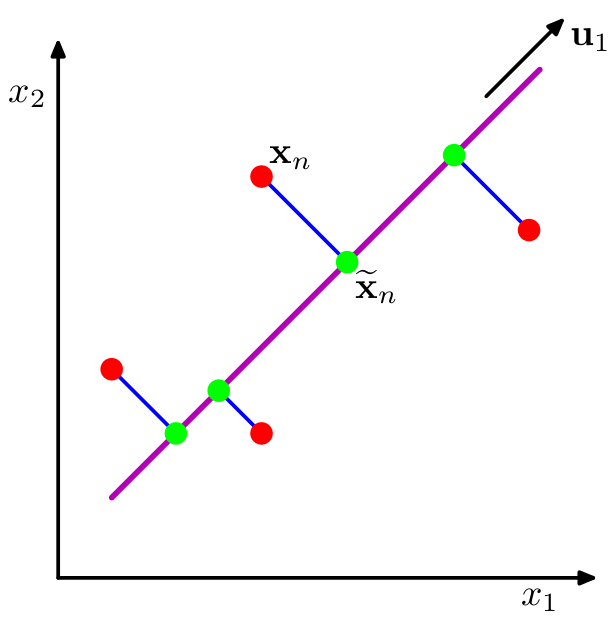
\includegraphics[width=0.5\textwidth]{pics/pca.png}
  \caption{ Orthogonal projection from two-dimensional space to one-dimensional subspace using PCA, where $u_1$ is the basis of the subspace, namely the principal component.}
\end{figure}

\subsection{PCA approximation}
\label{PCA approximation}
Once the data is projected onto a subspace, we can recover an approximation $\hat{x}$ of the data in the form
\begin{equation}
\label{pcaeq1}
	\hat{x} = \sum\limits_{i=i}^ku_i(u_i^Tx).
\end{equation}
where $k$ is the dimensionality of the subspace. Thus the value of the last $m-k$ dimensions will be approximated by zero. Since $u_i^Tx$ is a scalar, $\hat{x}$ would be a linear combination of the basis vectors.


Recall from \ref{sec:Auto-encoders}, auto-encoders can generate a hidden representation of data. If the number of hidden units is less than the dimensionality of the input data, this process can also be interpreted as  
dimensionality reduction. It is shown that if no nonlinear activation functions are used in auto-encoders, PCA essentially gives the optimal solution of auto-encoders in such cases. In other words, auto-encoders are nonlinear generalizations of PCA~\cite{hinton2006reducing}.

\subsection{Whitening}
\label{Whitening}
Whitening refers to the normalization of data to give it zero mean and same variance, so that different variables become less correlated. One way of achieving unit variance can be done based on PCA by rescaling each dimension of the projected data in the form of
\begin{equation}
\label{pcaeq2}
	w_i = \frac{u_i^Tx}{\sqrt{\lambda_i}}
\end{equation}
where $\lambda_i$ is the corresponding eigenvalue of $u_i$.

Moreover, if we multiply the whitened data $W$ by an orthogonal matrix, the property of unit variance will not be affected. Therefore, if we multiply $W$ by $U$ and keep all $n$ dimensions of the data, we will get the whitened version of data that is  as close as possible to the original data. Such process is called ZCA whitening, which is an important pre-processing step for many algorithms including convolutional neural networks.

\section{Markov Random Fields}
\label{sec:Markov Random Fields}
In many cases, a set of features or a set of data points are not independent of each other. Capturing such independencies is essential for building reasonable models. Probabilistic graphical models can be used to make assumptions about conditional independencies among the data set, and Markov random fields (MRF) are a type of probabilistic graphical models that are of particular interests in our study.

\subsection{Probabilistic graphical models}
\label{sec:Probabilistic graphical models}
Probabilities serve as the foundation of statistical machine learning. Numerous models are built based on different probabilistic assumptions. Probabilistic graphical models offer a way of expressing conditional independence properties via a graph, where its underlying mathematical expressions can be derived accordingly.

In a probabilistic graphical model, we used nodes to represents random variables, and edges to express probabilistic relationships between these variables. It constructs a general way of decomposing the joint distribution over all of the random variables into a product of factors, so that each depending only on a subset of the variables.

\subsection{Markov random fields}
\label{sec:Markov random fields}
Markov random fields are probabilistic graphical models with undirected edges, which is a more natural way of assigning probabilistic relationships than directed graphs in the cases where there is no obvious causal relationships.

If an edge exists between any pair of nodes in a subset of the graph, that set of nodes is called a clique. Every variable from a clique then is dependent of all the other variables in that clique. If no other nodes can be included in a clique, the it is called a maximal clique. 

The joint distribution can be written as a production of factors
\begin{equation}
	p(x) = \frac{1}{Z}\prod\limits_{C}\psi_C({x_C})
\end{equation}
where $x$ is an assignment of the graph, $\psi_C({x_C})$ is the potential function defined over a maximal clique, and $Z$ is a normalization constant so that 
\begin{equation}
	\int p(x)\mathrm{d}x = 1.
\end{equation}

\subsection{Energy function}
\label{sec:Energy function}

A convenient way of defining the potential functions is by using energy functions $E({x_C})$ over maximal cliques in the following form, so that the joint probability follows the Boltzmann distribution. 
\begin{equation}
\label{energy}
	\psi_C({x_C}) = \mathrm{exp}\{-E({x_C})\}
\end{equation}
Consequently, an assignment of $x_C$ has a high probability if the energy of that clique is low. Moreover the total energy of the joint distribution equals to the summation of the energies of each maximal clique.

\subsection{Image denoising}
\label{sec:Image denoising}
Markov random fields can be used for image denoising. Given a noisy image, our goal is to recover the original image based on the probabilistic relationships assumed by Markov random fields. 

More specifically, for a $m$ by $n$ noisy image, we first use $m\times n$ nodes to represent all the pixels. Since we already knew the value of  each pixels, such set of nodes are called observed nodes. Then we use another set of $m\times n$ latent nodes to represent the noiseless image we want to recover, whose values are unknown. An edge is assigned between each pair of latent and observed nodes, denoting some extent of consistency between the noisy and original image. Edges are also constructed between neighbouring latent nodes, which indicates their values are correlated. An illustration of such Markov random fields given by~\cite{bishop2006pattern} is shown in Figure \ref{mrffig}.

\begin{figure}[h!]
  \centering
  \label{mrffig}
  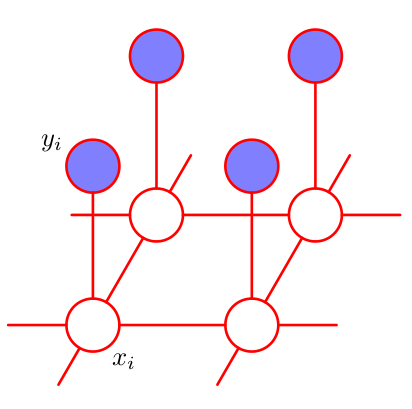
\includegraphics[width=0.4\textwidth]{pics/mrf.png}
  \caption{ An example Markov random fields for image denoising, $y_i$ is a an observed node and $x_i$ is a latent node.}
\end{figure}

To ensure the above probabilistic relationships, we need to construct energy functions that returns a smaller value if nodes in a clique agree with each other and returns a greater value if not. Thus the latent nodes with the highest probability will prefer similar values in a neighbourhood and at the same time being consistent with the observed nodes to some extent as well. Therefore such latent nodes are likely to a good estimation of the original noiseless image.
 
In order to reach the state of the lowest energy, we can use the max-product algorithm on factor graphs. However, the construction of factor graphs is difficult if the structure of MRF is allowed to be mutable. For discrete variables, a local search algorithm called iterated conditional modes can be applied on an arbitrary structure is more suitable to our needs~\cite{kittler1984contextual}.

We can further extend this app latent nodes to any given graph with observed assignments as long as they satisfy the properties of Markov random fields.


\section{Image Segmentation}
\label{sec:Image Segmentation}

Image segmentation is the task of splitting images into groups of pixels that share similar attributes (e.g., belong to the same semantic object). Since an image can be segmented in different manners, hundreds of algorithms are studied for various requirements~\cite{szeliski2010computer}. In our study, we are particularly interested in segmenting images into super-pixels, so that the pixels within the same group are visually similar but not semantically meaningful.

\subsection{Graph-based segmentation}
\label{sec:Graph-based segmentation}

Images can be represented by a graph where each pixel corresponds to a node and edges are established between adjacent pixels. While many algorithms use a fixed criterion to decide similarities between pixels or regions, an algorithm that employs a relative measure of evidence for a boundary between two regions is shown to be of great practical importance~\cite{felzenszwalb2004efficient}.

If we use graph $G$ to represent an image, then a region $R$ of the image is essentially a connected component of graph $G$. Let $MST(R)$ be all the edges in a minimum spanning tree of $R$. The algorithm uses $Int(R)$ to evaluate the internal difference for any region $R$, which is given by
\begin{equation}
	Int(R) = \max\limits_{e\in MST(R)}w(e)
\end{equation}
where $w(e)$ is the weight of the edge. In terms of image segmentation, it should be the measure of the dissimilarity between the two pixels connected by that edge (e.g., the difference in intensity,
color).

The difference between two regions $R_1$ and $R_2$ is measured by the weight of the shortest edge connecting two regions, in the form of
\begin{equation}
	Dif(R_1,R_2) = \min\limits_{v_1\in R_1, v_2\in R_2}w(v_1,v_2).
\end{equation}

The algorithm will merge to disconnected regions if $Dif(R_1,R_2)$ is greater than the minimum value of $Int(R_1)$ and $Int(R_2)$. In other to adjust the evidence of a boundary as we need, a threshold function $\tau$ is often added to the minimum values. So that the minimum internal difference of $R_1$ and $R_2$ becomes
\begin{equation}
	MInt(R_1,R_2) = \min((Int(R_1)+\tau(R_1)),(Int(R_2)+\tau(R_2))).
\end{equation}

Such operations can be performed efficiently using disjoint sets, the running time hence is linear with regard to the number of pixels in practice. Super-pixels generated by the graph-based segmentation can be guaranteed to be neither to coarse or to fine~\cite{felzenszwalb2004efficient}. It has many pragmatic applications, including the 3D reconstruction method we are going to discuss in Section \ref{sec:3D Reconstruction}. An example result using graph-based segmentation on a road scene image is shown in Figure \ref{gsuperfig}.

\begin{figure}[h!]
\centering
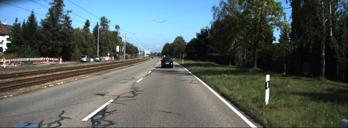
\includegraphics[width=0.7\linewidth]{pics/super1.jpg}
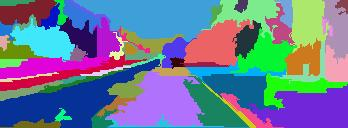
\includegraphics[width=0.7\linewidth]{pics/super2.jpg}
\caption{Super-pixels (bottom) of a road scene image (top) generated by graph based image segmentation.}
\label{gsuperfig}
\end{figure}

\subsection{Simple linear iterative clustering}
\label{sec:Simple linear iterative clustering}
One important limitation of the graph-based segmentation algorithm is it does not engage spatial regularization properties, since the weights of edges in a graph only depend on the colour and intensity attributes of connected pixels. Many applications prefer super-pixels that are regular and compact in shapes as they can be considered as a good abstraction of images. 

In the simple linear iterative clustering (SLIC) algorithm, pixels are consider as points in a five-dimensional space, which is a combination of a three-dimensional color space and a two-dimensional spatial plane. By utilizing the spatial information of pixels, it offers an adaptable degree of regularization in shapes of super-pixels.

In the SLIC algorithm we often represent images using the Lab colour space, therefore the distance between two pixels in the five-dimensional space is given by
\begin{equation}
	d(p_1,p_2) = \sqrt{(\frac{d_c}{n_c})^2,(\frac{d_s}{n_s})^2}
\end{equation}
where $n_c$ and $n_s$ are spatial regularization terms, $d_c$ is the Euclidean distance in colour space in the form of 
\begin{equation}
	d_c(p_1,p_2) = \sqrt{(l_1-l_2)^2,(a_1-a_2)^2,(b_1-b_2)^2}
\end{equation}
and $d_s$ is the Euclidean distance in spatial plan in the form of
\begin{equation}
	d_s(p_1,p_2) = \sqrt{(x_1-x_2)^2,(y_1-y_2)^2}.
\end{equation}

The SLIC algorithm then performs a clustering algorithm based on iterative improvement described in~\cite{achanta2012slic}. As suggested by its name, the running time of this algorithm is shown to be linear in practice.

\section{3D Reconstruction}
\label{sec:3D Reconstruction}
The task of reconstructing 3D models from a set of images is call 3D Reconstruction. It has substantive practical applicability, and many algorithms as been devised for this purpose. However most of the algorithms require two or more images taken from the same scenario, which is not suitable for our purpose.

A different approach to infer 3D structure was introduced as part of the  ``Photo Pop-up'' application by~\cite{hoiem2005automatic}. Instead of using widely applied multiple view geometry methods, this approach engages statistical machine learning methods to train a classifier. It requires only a single image, can assign each part of the image into one of three basic geometric categories, namely ``ground'', ``vertical'' and ``sky''. 

In the training step, a image will be segmented into super-pixels using the graph-based segmentation described in \ref{sec:Graph-based segmentation}. Then for one super-pixel, a set of features (including colour, texture, location, shapes, lines, intersections etc.) are extracted. A statistical model for classification is trained on a set of manually labeled images. 

In the prediction step, an image will be first segmented into super-pixels. Then a label for each super-pixels can be obtained via the trained classifier. Finally they will be grouped into plausible regions in a way such that super-pixels within the same group are of high probability of belonging to the same geometric category. A elaborated description and sample outputs (Figure \ref{3Dfig}) of the algorithm and its theoretical background is provided in~\cite{hoiem2005automatic}.

\begin{figure}[h!]
\centering
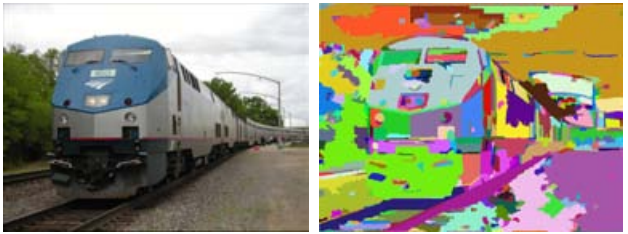
\includegraphics[width=0.8\linewidth]{pics/3d1.png}
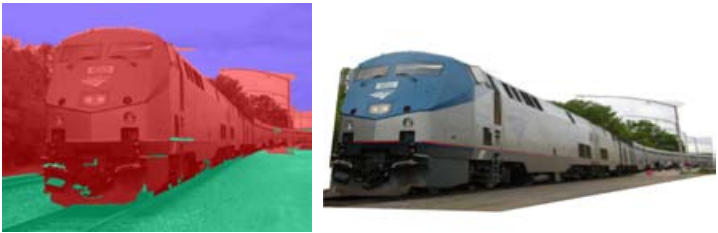
\includegraphics[width=0.8\linewidth]{pics/3d2.png}
\caption{Sample input image (top left), segmentation result (top right), labeling result (bottom left) and 3D view (bottom right) of the ``Photo Pop-up'' application.}
\label{3Dfig}
\end{figure}
